\chapter{Benchmark results}
%% Pentium4 3GHz, 1GB RAM, 800MHz 533MHz DDR
All benchmarks was tested on the same machine which makes the comparison more 
acurate. The benchmarking computer was Pentium 4 on 3GHz with 1GB RAM running
Debian 4.0 Linux with kernel 2.6.18. Solvers were tested in folloving versions:
\begin{itemize}
\item SICStus Prolog -- 4.0.4/glibC 2.3
\item \eclipse -- 4.0.4/glibC 2.3
\item Mozart - 1.3.2 (20061204), version from Debian packages system 
\item Minion -- 0.7RC1, svn version 1258
\item Gecode -- 2.1.1
\end{itemize}

\begin{figure}[Table]
\caption{Tabulka 1}
\begin{tabular}{lrrr}
\hline \itshape Solver	&	 \itshape Time first	&	\itshape Time all & \itshape Speedup \\
\hline Minion	&	 31.6 & *To be measured* & *To be measured * \\
\hline
\end{tabular}
\end{figure}

\begin{figure}
\begin{center}
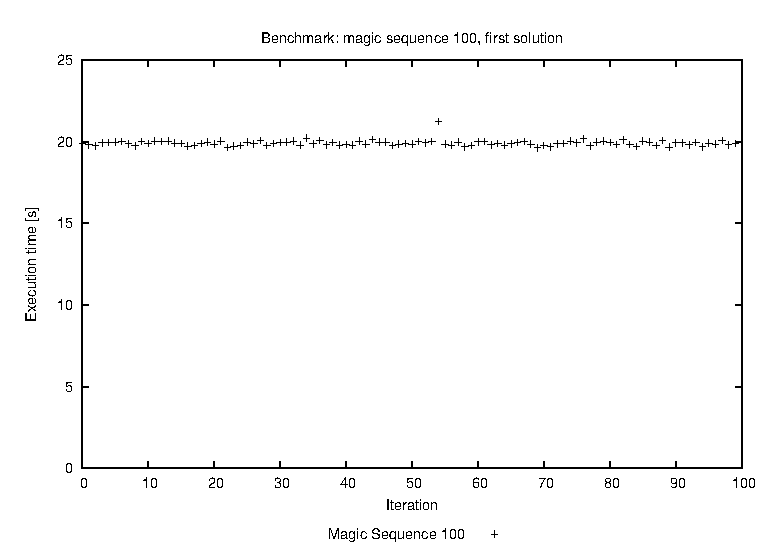
\includegraphics[width=8cm]{images/grafy/100magic.eps}
\end{center}
\end{figure} 
